\documentclass[tikz,border=8pt]{standalone}
\usepackage{amsmath,amssymb}
\usetikzlibrary{arrows.meta,automata,positioning,quotes}
\begin{document}
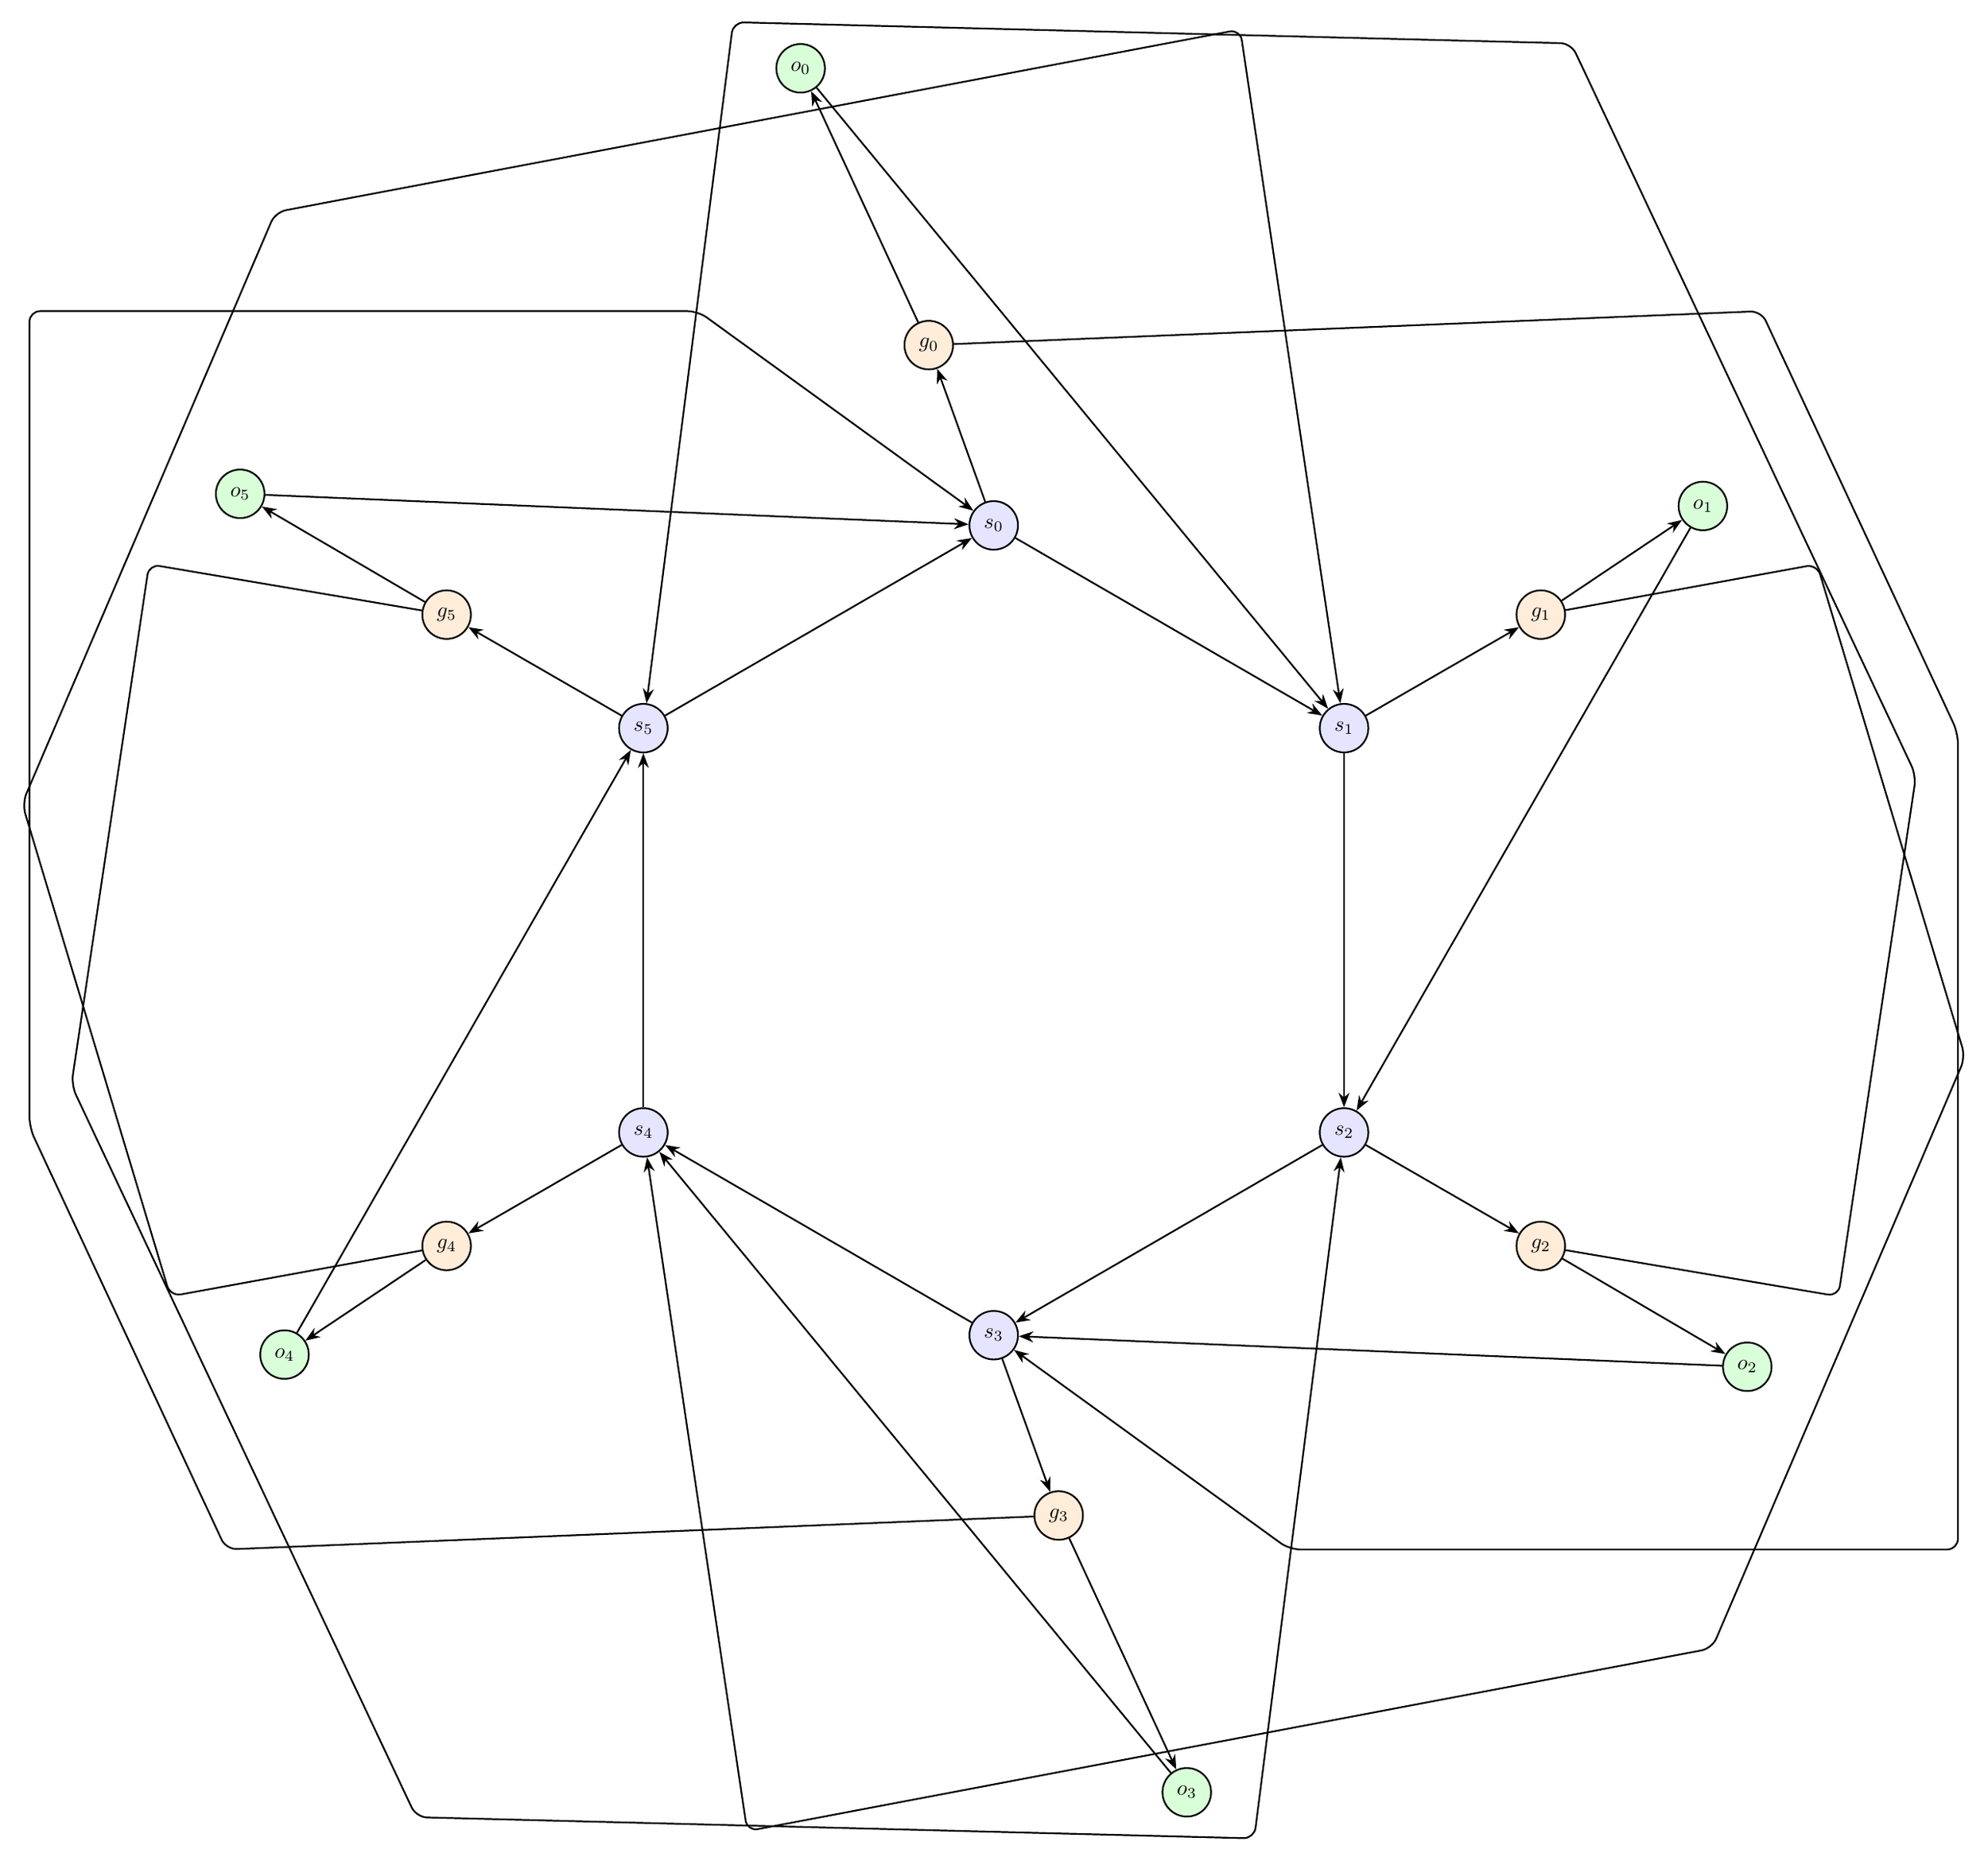
\begin{tikzpicture}[x=1cm,y=1cm]
\tikzset{
  graphnode/.style={circle,draw,thick,minimum size=8mm,inner sep=1pt,font=\sffamily},
  directed/.style={-{Stealth[length=2.4mm]},thick},
  undirected/.style={thick}
}
\node[graphnode,fill=blue!10] (n_s0) at (0.00,6.67) {$s_0$};
\node[graphnode,fill=blue!10] (n_s1) at (5.77,3.33) {$s_1$};
\node[graphnode,fill=blue!10] (n_s2) at (5.77,-3.33) {$s_2$};
\node[graphnode,fill=blue!10] (n_s3) at (0.00,-6.67) {$s_3$};
\node[graphnode,fill=blue!10] (n_s4) at (-5.77,-3.33) {$s_4$};
\node[graphnode,fill=blue!10] (n_s5) at (-5.77,3.33) {$s_5$};
\node[graphnode,fill=orange!15] (n_g0) at (-1.07,9.64) {$g_0$};
\node[graphnode,fill=orange!15] (n_g1) at (9.01,5.20) {$g_1$};
\node[graphnode,fill=orange!15] (n_g2) at (9.01,-5.20) {$g_2$};
\node[graphnode,fill=orange!15] (n_g3) at (1.07,-9.64) {$g_3$};
\node[graphnode,fill=orange!15] (n_g4) at (-9.01,-5.20) {$g_4$};
\node[graphnode,fill=orange!15] (n_g5) at (-9.01,5.20) {$g_5$};
\node[graphnode,fill=green!15] (n_o0) at (-3.18,14.20) {$o_0$};
\node[graphnode,fill=green!15] (n_o1) at (11.68,6.99) {$o_1$};
\node[graphnode,fill=green!15] (n_o2) at (12.41,-7.19) {$o_2$};
\node[graphnode,fill=green!15] (n_o3) at (3.18,-14.20) {$o_3$};
\node[graphnode,fill=green!15] (n_o4) at (-11.68,-6.99) {$o_4$};
\node[graphnode,fill=green!15] (n_o5) at (-12.41,7.19) {$o_5$};
\draw[directed] (n_s0) -- (n_s1);
\draw[directed] (n_s1) -- (n_s2);
\draw[directed] (n_s2) -- (n_s3);
\draw[directed] (n_s3) -- (n_s4);
\draw[directed] (n_s4) -- (n_s5);
\draw[directed] (n_s5) -- (n_s0);
\draw[directed] (n_s0) -- (n_g0);
\draw[directed] (n_g0) -- (n_o0);
\draw[directed] (n_o0) -- (n_s1);
\draw[directed] (n_s1) -- (n_g1);
\draw[directed] (n_g1) -- (n_o1);
\draw[directed] (n_o1) -- (n_s2);
\draw[directed] (n_s2) -- (n_g2);
\draw[directed] (n_g2) -- (n_o2);
\draw[directed] (n_o2) -- (n_s3);
\draw[directed] (n_s3) -- (n_g3);
\draw[directed] (n_g3) -- (n_o3);
\draw[directed] (n_o3) -- (n_s4);
\draw[directed] (n_s4) -- (n_g4);
\draw[directed] (n_g4) -- (n_o4);
\draw[directed] (n_o4) -- (n_s5);
\draw[directed] (n_s5) -- (n_g5);
\draw[directed] (n_g5) -- (n_o5);
\draw[directed] (n_o5) -- (n_s0);
\draw[directed,rounded corners=5pt] (n_g0) -- (12.64,10.20) -- (15.88,3.25) -- (15.88,-10.20) -- (4.87,-10.20) -- (n_s3);
\draw[directed,rounded corners=5pt] (n_g1) -- (13.56,6.03) -- (16.00,-2.09) -- (11.83,-11.83) -- (-4.06,-14.84) -- (n_s4);
\draw[directed,rounded corners=5pt] (n_g2) -- (13.91,-6.03) -- (15.19,2.55) -- (9.51,14.61) -- (-4.29,14.96) -- (n_s5);
\draw[directed,rounded corners=5pt] (n_g3) -- (-12.64,-10.20) -- (-15.88,-3.25) -- (-15.88,10.20) -- (-4.87,10.20) -- (n_s0);
\draw[directed,rounded corners=5pt] (n_g4) -- (-13.56,-6.03) -- (-16.00,2.09) -- (-11.83,11.83) -- (4.06,14.84) -- (n_s1);
\draw[directed,rounded corners=5pt] (n_g5) -- (-13.91,6.03) -- (-15.19,-2.55) -- (-9.51,-14.61) -- (4.29,-14.96) -- (n_s2);
\end{tikzpicture}
\end{document}
